\section{Descripción experimental}

El montaje consiste en una cámara que tiene una abertura sobre la cual se coloca la muestra en forma de placa, sobre esta se coloca un bloque de hielo \ref{fig:montaje}. En primer lugar, se mide qué tan rápido se funde el hielo debido al intercambio de calor con el medio ambiente, luego de tener esta tasa, se procede a conectar la cámara a la fuente de vapor, y luego de que se satura, se mide la tasa de fusión del hielo debido a la diferencia de temperatura.


\begin{figure}[t]
    \centering
    \begin{subfigure}[b]{0.45\textwidth}
        \centering
        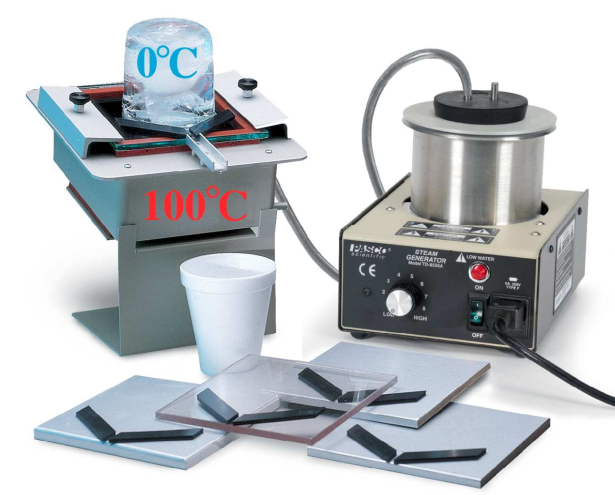
\includegraphics[width=1\linewidth]{img/montaje.png}
        \caption{Montaje usado. Tomado de  \cite{conductividad_notas}}
        \label{fig:montaje_a}
    \end{subfigure}
    \begin{subfigure}[b]{0.45\textwidth}
        \centering
        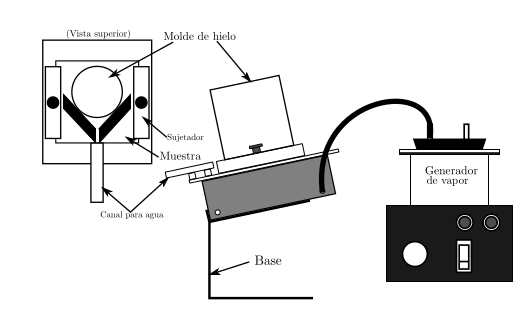
\includegraphics[width=\linewidth]{img/montaje_vista_lateral.png}
        \caption{Vista lateral esquematica del montaje. }
        \label{fig:montaje_b}
    \end{subfigure}
    \caption{Foto y esquema del montaje. Tomado de  \cite{conductividad_notas}}
\end{figure}
El equipo a utilizar consta de las siguientes partes \cite{conductividad_notas}:
\begin{itemize}
    \item base
    \item cámara de vapor,
    \item generador de vapor
    \item molde de hielo
    \item Muestras de diferentes materiales.
\end{itemize}